\documentclass[handout,aspectratio=169]{beamer}
\setbeamertemplate{section in toc}[sections numbered]

\usetheme[numbering=fraction]{metropolis}
\metroset{block=fill}
\usepackage{appendixnumberbeamer}
\usepackage[export]{adjustbox}
\usepackage{nicefrac}
\usepackage{subcaption}
\usepackage{tabularx}
\usepackage{booktabs}
\usepackage[scale=2]{ccicons}

\usepackage{xspace}
\newcommand{\themename}{\textbf{\textsc{metropolis}}\xspace}

\title{Bursting the Burden Bubble?}
\subtitle{An Assessment of Sharma et al.'s Counterfactual-Based Fairness Metric}
\date{\textit{November 8, 2022}}
\author{%
Yochem van Rosmalen {\scriptsize(\texttt{y.m.vanrosmalen@students.uu.nl})}\\
Florian van der Steen {\scriptsize(\texttt{f.a.vandersteen@students.uu.nl})}\\
Sebastiaan Jans {\scriptsize(\texttt{s.j.j.jans@students.uu.nl})}\\
Daan van der Weijden {\scriptsize(\texttt{d.j.weijden@students.uu.nl})}
}
\institute{Utrecht University, The Netherlands}
\titlegraphic{\hfill
\includegraphics[height=1.5cm]{img/uu_logo.png}}

\begin{document}

\maketitle

\begin{frame}{Outline}
    \tableofcontents
\end{frame}

\section{Fairness}

\begin{frame}{Fairness}
    \begin{columns}
        \begin{column}{0.5\textwidth}
            \begin{itemize}
            \item What is fairness?
            \item Many aspects of fairness \pause \alert{metrics}
            \end{itemize}
        \end{column}
        \begin{column}{0.5\textwidth}
            \begin{figure}
                \centering
                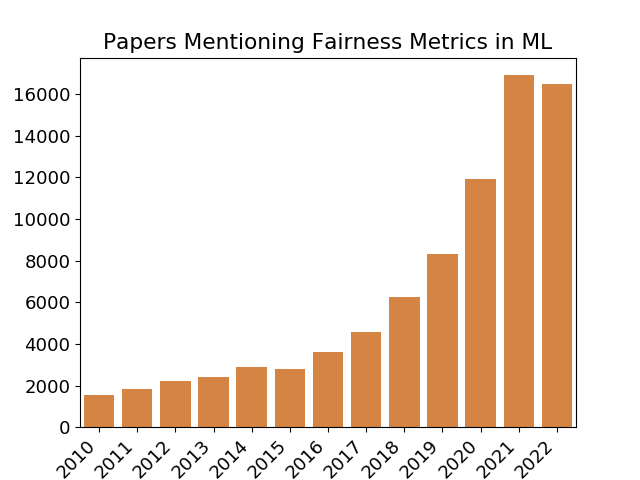
\includegraphics[width=\textwidth]{img/fairness.png}
                \label{fig:fairnessmetrics}
            \end{figure}
        \end{column}
    \end{columns}
\end{frame}

\subsection{Statistical Parity}
\begin{frame}{Statistical Parity}

\begin{columns} 
    \begin{column}{.5\textwidth}

        Statistical/Demographic Parity 
 ($SP_S$) \cite{hardt2016equalisedodds}: Ratio of acceptance rates ($AR_S$).

        \begin{equation*}
            SP_{S} = \frac{AR_{S=A}}{AR_{S=B}} = \frac{P(\hat{Y}=1|S=A)}{P(\hat{Y}=1|S=B)} 
        \end{equation*}
        
        Perfect parity: $SP_S = 1$
        
        % Acceptable parity: $SP_S \geq 0.8$
        
        80\% rule \cite{feldman2015certifying}: $SP_S \geq 0.8$ is acceptable.

    \end{column}
    
    \begin{column}{.5\textwidth}
    \begin{center}
        \begin{figure}
            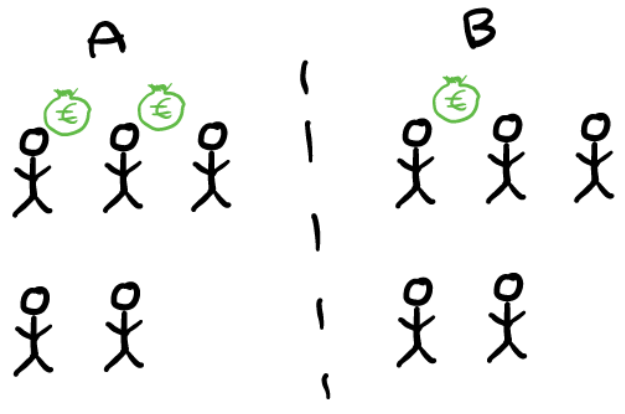
\includegraphics[width=.8\textwidth]{img/no_parity.png}
            % \caption{No Parity}
            % \label{fig:no-parity}
        \end{figure}
        $\frac{1/5}{2/5} = 0.5 < 0.8$
        
        \alert{No parity!}
    \end{center}
        
    \end{column}
    

    \renewcommand{\thefootnote}{\fnsymbol{footnote}}
    \footnotetext[0]{$\hat{Y}$: Model's prediction, $S$: Sensitive attribute/group}
    
    
\end{columns}
\end{frame}

\subsection{Burden}

\begin{frame}{Burden}
    \begin{columns}
        \begin{column}{0.5\textwidth}
            \begin{itemize}
                \item Sharma et al.'s CERTIFAI framework \cite{certifai} (2017)
                \item CognitiveScale
                \item Multiple domains
                \item Model Agnostic
                \item Counterfactuals
                \begin{itemize}
                    \item \alert{Not causal!}
                    \item Generated with genetic algorithm
                \end{itemize}
            \end{itemize}
        \end{column}
        \begin{column}{0.5\textwidth}
            \begin{figure}
                \centering
                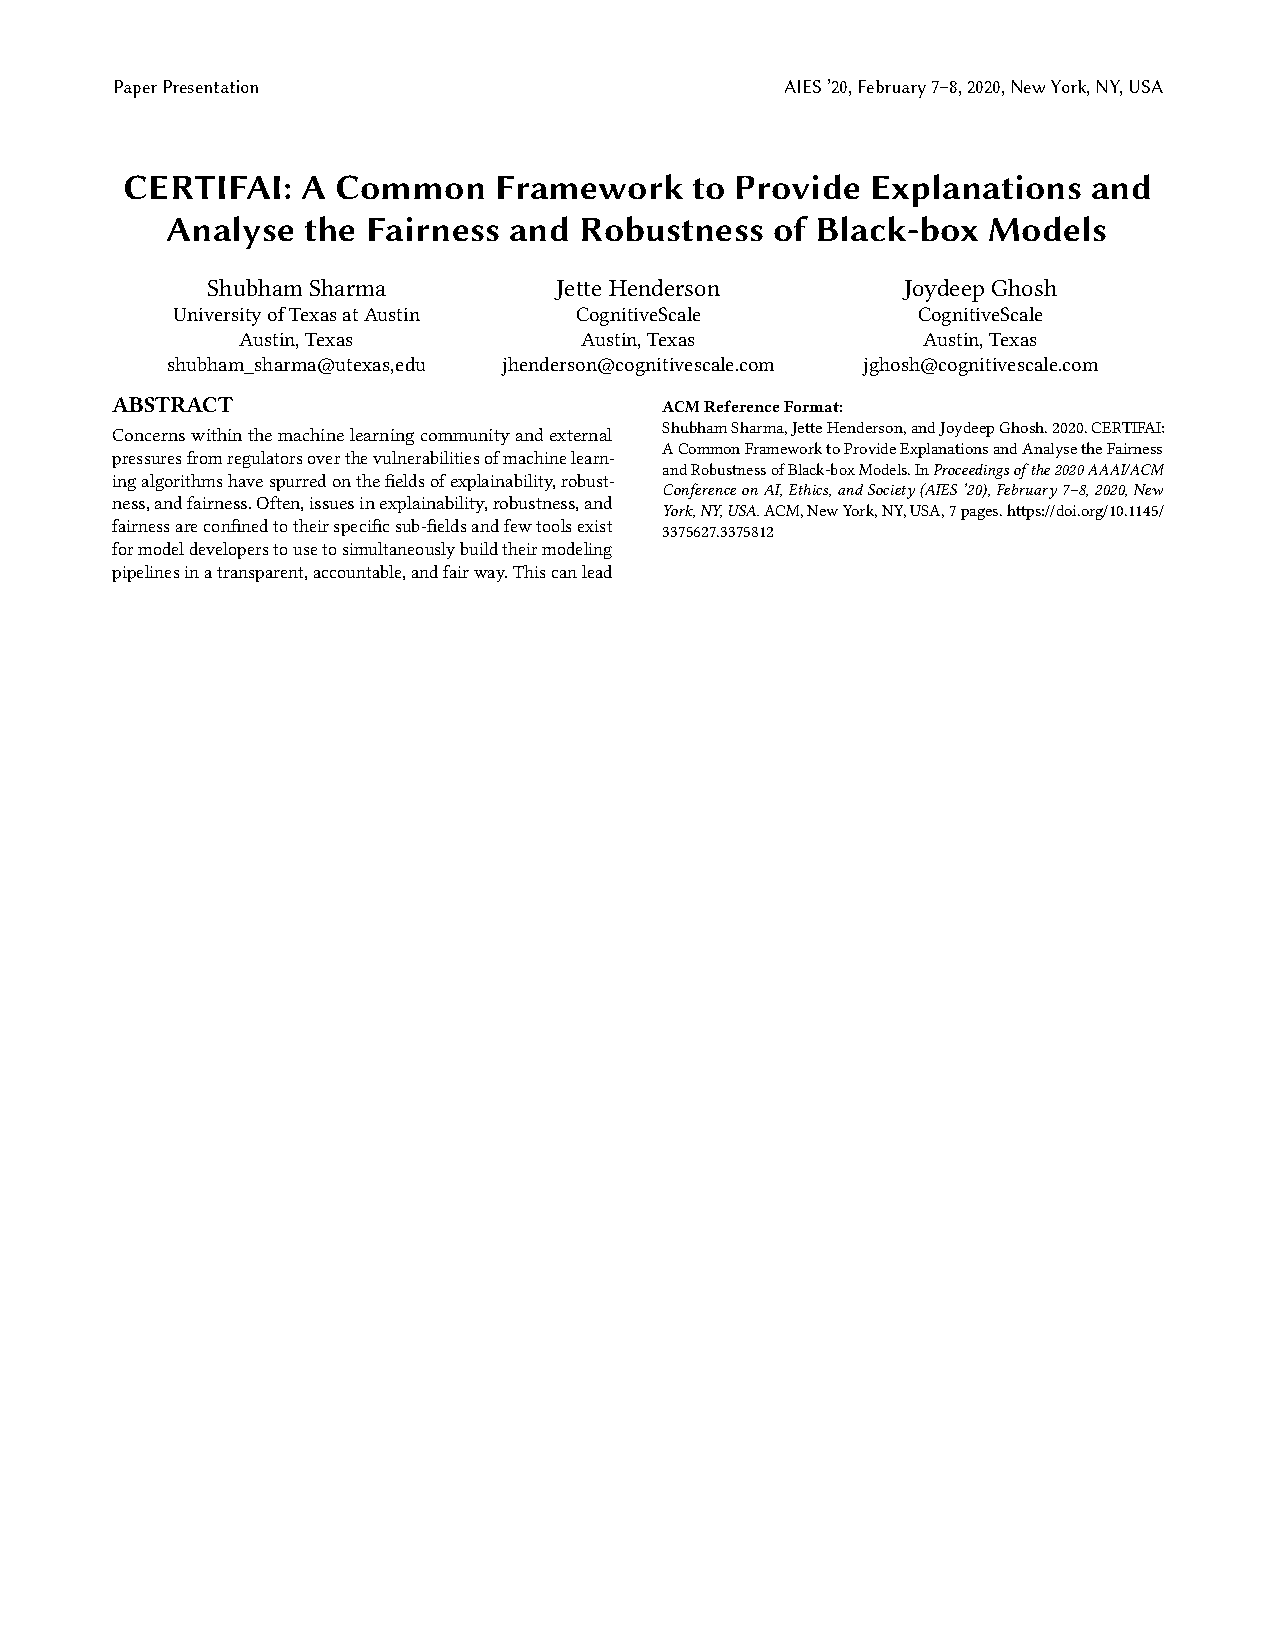
\includegraphics[width=\textwidth]{img/certifai.pdf}
            \end{figure}
        \end{column}
    \end{columns}
    
\end{frame}

\begin{frame}{Counterfactual generation}
    \begin{figure}
    \centering
    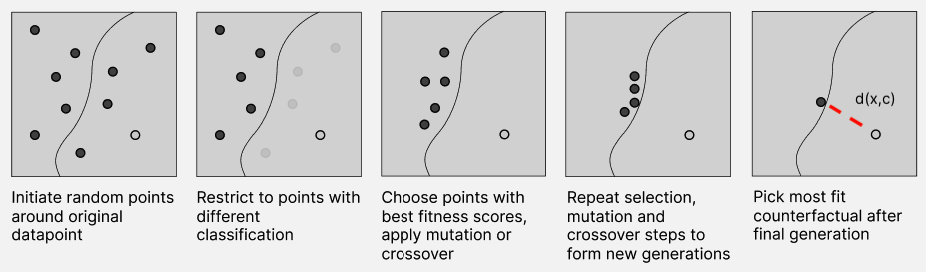
\includegraphics[width=\textwidth]{img/counterfactual_generation_burden.png}
    \end{figure}
    Evolutionary algorithm for the generation of realistic counterfactuals. Illustration adapted from \cite{certifai}.
\end{frame}

\begin{frame}{Burden}
    \begin{itemize}
        \item Distance to counterfactual \textrightarrow individual \emph{recourse}.
        \item Average distance to counterfactual over instances in a group $s$, with $\mathbf{c^*}$ the found counterfactual(s):
    \end{itemize}
    \begin{align*}\label{eq:burden}
        \text{Burden}_{S=s} &= \mathbb{E}_{S=s}[d(\mathbf{x}, \mathbf{c^*})] \\
        % &= \frac{1}{|s|} \sum_{x \in s} d(\mathbf{x}, \mathbf{c^*})
    \end{align*}
\end{frame}


\section{Experiments}
\subsection{Synthetic Datasets}

\begin{frame}{Synthetic datasets}
\begin{itemize}
    \item Goal: Highlighting theoretical difference between metrics
    \item What the metrics measure:
    \begin{itemize}
        \item Burden: Estimated \alert{distance} to counterfactual
        \item SP: \alert{Rate} of favorably classified
    \end{itemize}
    \item Approach:
    \begin{itemize}
        \item Dataset $D_A$: $AR_{S=0} = AR_{S=1}$, $\text{Burden}_{S=0} > \text{Burden}_{S=1}$ 
        \item Dataset $D_B$: $AR_{S=0} > AR_{S=1}$, $\text{Burden}_{S=0} < \text{Burden}_{S=1}$ 
    \end{itemize}
\end{itemize}
\end{frame}

\begin{frame}{Results Synthetic Datasets}
\begin{figure}
    \centering
    \begin{subfigure}{0.49\textwidth}
        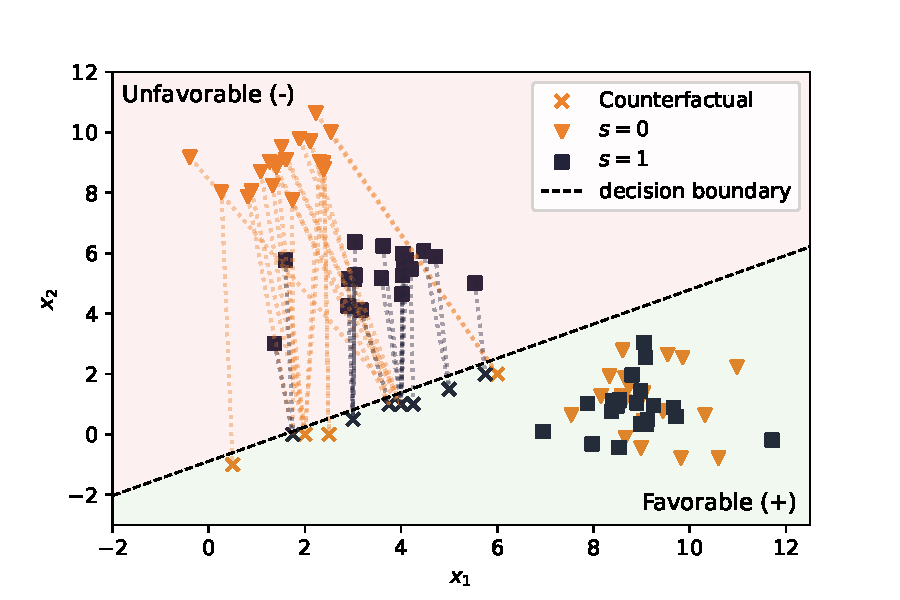
\includegraphics[width=\textwidth]{img/syndata-A}
        \caption{$D_A$, where Burden and statpar \\ disagree on the presence of unfairness.}
        \label{fig:syndatafavor}
    \end{subfigure}
    \begin{subfigure}{0.49\textwidth}
        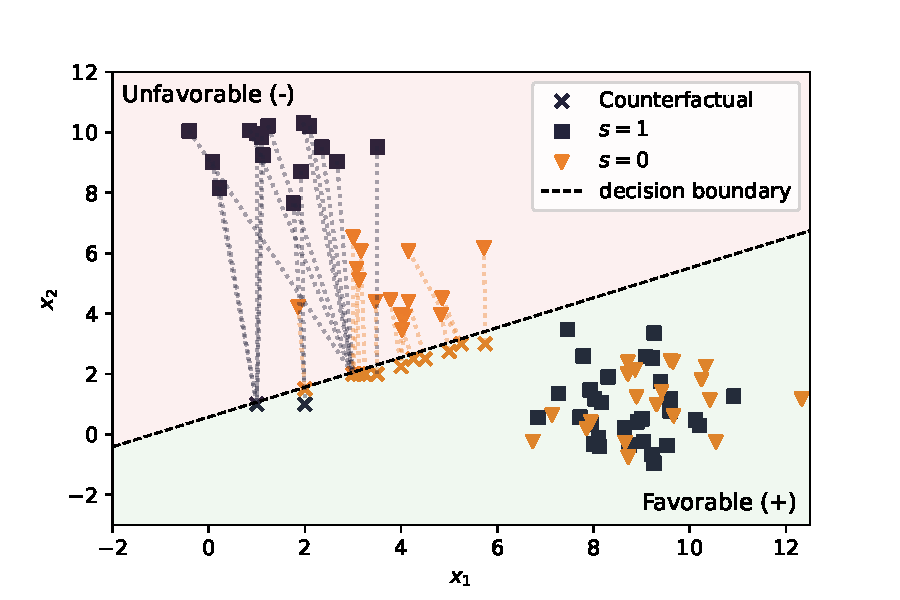
\includegraphics[width=\textwidth]{img/syndata-B}
        \caption{$D_B$, where Burden and statpar \\ disagree on the direction of unfairness.}
        \label{fig:syndataunfavor}
    \end{subfigure}
\end{figure}
\end{frame}

\subsection{Taiwan Dataset}
    
\begin{frame}{Real world dataset}
    \begin{itemize}
        \item Default of Credit Card Clients Data Set, ``Taiwan'' \cite{dataset}
        \begin{itemize}
            \item Target: did the person default on loan?
            \item 30,000 instances (1000 counterfactuals)
            \item 4 Sensitive attributes (dropped for training)
            \item All features concerning account balances 
        \end{itemize}
        \item Logistic Regression with 78\% accuracy
    \end{itemize}    
\end{frame}

\begin{frame}{Results}
    \begin{table}
    \centering
    \label{table:results}
    \begin{tabularx}{.8\textwidth}{l@{\extracolsep{\fill}}cccccc}
    % \toprule
    & \multicolumn{2}{c}{Acceptance Rate} & SP & \multicolumn{3}{c}{Burden}\\
    \cmidrule(lr){2-3}\cmidrule(lr){4-4}\cmidrule(lr){5-7}
    % & \multicolumn{2}{c}{$S$} & ratio  & \multicolumn{2}{c}{$S$} & ratio\\
    % \cmidrule(lr){2-3}\cmidrule(lr){4-4}\cmidrule(lr){5-6}\cmidrule(lr){7-7}
    Dataset & $S=0$ & $S=1$ & 0/1 & $S=0$ & $S=1$ & 0/1\\
    \midrule
    
    $D_A$  & 0.500 & 0.500 & 1.00 & \textbf{11.6} & 4.65 & 2.49\\
    $D_B$  & \textbf{0.571} & 0.667 & 0.857 & 3.31 & \textbf{11.0} & 0.302\\
    Taiwan & 0.967 & \textbf{0.948} & 1.02 & \textbf{1.38} & 0.940 & 1.47\\
    \bottomrule
    \end{tabularx}
\end{table}
Underprivileged group according to metric in \textbf{boldface}.

For Taiwan: 0 is women, 1 is men.
\end{frame}

\section{Conclusions}

\begin{frame}{Conclusions}
    \begin{itemize}
        \item Burden can provide more nuance than Statistical Parity
        \item Computational cost of Burden is high
        % \item Use both when possible 
        \item Burden can be used in addition to Statistical Parity
    \end{itemize}

    \vspace{1cm}
    \begin{center}
    {\large\alert{Concluding, be mindful when using a single fairness metric!}}
    \end{center}
\end{frame}

\section{Future Work}
\begin{frame}{Future Work}
    \begin{itemize}
        \item Reduce computational complexity of Burden
        \item Find real-world datasets with SP and Burden disagree on the direction of unfairness
    \end{itemize} 
\end{frame}

\appendix

\begin{frame}[standout]
  Questions?
\end{frame}

\begin{frame}[allowframebreaks]{References}
% \begin{frame}{References}

  \bibliography{references}
  \bibliographystyle{abbrv}

\end{frame}


\begin{frame}{Find the slides, paper and code on GitHub!}

\begin{center}
    
\includegraphics[width=.6\textwidth]{img/github.png}
    \vspace{1cm}
    \alert{
    \href{https://github.com/yochem/bursting-burden}{github.com/yochem/bursting-burden}
    }
\end{center}
\end{frame}

\end{document}
